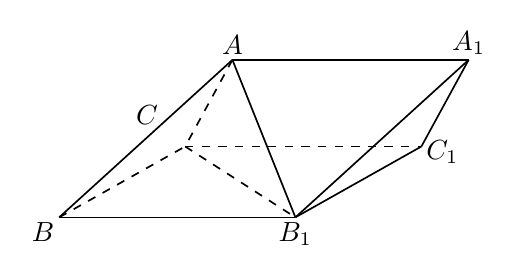
\begin{tikzpicture}[x=1cm,y=1cm,line width=0.6pt]
  \coordinate (B) at (0,0);
  \coordinate (B1) at (3.0,0);
  \coordinate (C) at (1.6,0.9);
  \coordinate (C1) at (4.6,0.9);
  \coordinate (A) at (2.2,2.0);
  \coordinate (A1) at (5.2,2.0);
  % bottom and top faces
  \draw[black,solid] (B) -- (B1);
  \draw[black,solid] (A) -- (A1);
  \draw[black,solid] (A) -- (B);
  \draw[black,solid] (A) -- (B1);
  \draw[black,solid] (B1) -- (A1);
  \draw[black,solid] (A1) -- (C1);
  \draw[black,solid] (B1) -- (C1);
  % dashed hidden edges
  \draw[black,dashed] (B) -- (C);
  \draw[black,dashed] (A) -- (C);
  \draw[black,dashed] (C) -- (C1);
  \draw[black,dashed] (C) -- (B1);
  \node[fill=white,inner sep=1.5pt,font=\normalsize,above] at (A) {$A$};
  \node[fill=white,inner sep=1.5pt,font=\normalsize,above] at (A1) {$A_{1}$};
  \node[fill=white,inner sep=1.5pt,font=\normalsize,below left] at (B) {$B$};
  \node[fill=white,inner sep=1.5pt,font=\normalsize,below] at (B1) {$B_{1}$};
  \node[fill=white,inner sep=1.5pt,font=\normalsize,above left,fill=none,xshift=-8.00bp,yshift=6.00bp] at (C) {$C$};
  \node[fill=white,inner sep=1.5pt,font=\normalsize,right,fill=none,xshift=0.00bp,yshift=-2.00bp] at (C1) {$C_{1}$};
\end{tikzpicture}
